\documentclass[a4paper,UTF8]{article}

\usepackage[margin=1.25in]{geometry}
\usepackage{color}
\usepackage{graphicx}
\usepackage{amssymb}
\usepackage{amsmath}
\usepackage{amsthm}
\usepackage{enumerate}
\usepackage{bm}
\usepackage{hyperref}
\usepackage{epsfig}
\usepackage{color}
\usepackage{mdframed}
\usepackage{lipsum}
\usepackage{mathtools}
\usepackage{algorithm}
\usepackage{algorithmic}
\usepackage{listings}
\usepackage{xcolor}
\usepackage{float}
\usepackage{caption}
\usepackage{mathrsfs}
\usepackage{amsmath}
\usepackage[utf8]{inputenc}
\usepackage[UTF8]{ctex}

\newmdtheoremenv{thm-box}{myThm}
\newmdtheoremenv{prop-box}{Proposition}
\newmdtheoremenv{def-box}{define}

\setlength{\evensidemargin}{.25in}
\setlength{\textwidth}{6in}
\setlength{\topmargin}{-0.5in}
\setlength{\topmargin}{-0.5in}

\usepackage{indentfirst}
\setlength{\parindent}{2em}

\usepackage{subfigure}
% \setlength{\textheight}{9.5in}
%%%%%%%%%%%%%%%%%%set header and footer here%%%%%%%%%%%%%%%%%%
\usepackage{fancyhdr}
\usepackage{lastpage}
\usepackage{layout}
\footskip = 10pt
\pagestyle{fancy}
\lhead{2020, Spring}
\chead{大数据综合处理实验}
\rhead{金庸的江湖——金庸武侠小说中的人物关系挖掘}
\cfoot{\thepage}
\renewcommand{\headrulewidth}{1pt}  			%header
\setlength{\skip\footins}{0.5cm}    			
\renewcommand{\footrulewidth}{0pt}  		

\makeatletter 							
\def\headrule{{\if@fancyplain\let\headrulewidth\plainheadrulewidth\fi%
\hrule\@height 1.0pt \@width\headwidth\vskip1pt	
\hrule\@height 0.5pt\@width\headwidth  			
\vskip-2\headrulewidth\vskip-1pt}      			
 \vspace{6mm}}     						
\makeatother

\graphicspath{{img/}}

\lstset{
 columns=fixed,
 basicstyle = \footnotesize,
 breakatwhitespace=false,         % 设置是否当且仅当在空白处自动中断.
 breaklines=true,
 numbers=left,                                        % 在左侧显示行号
 numberstyle=\tiny\color{gray},                       % 设定行号格式
 frame=none,                                          % 不显示背景边框
 backgroundcolor=\color[RGB]{245,245,244},            % 设定背景颜色
 keywordstyle=\color[RGB]{40,40,255},                 % 设定关键字颜色
 numberstyle=\footnotesize\color[RGB]{96,96,96},
 commentstyle=\color[RGB]{0,128,0},                % 设置代码注释的格式
 stringstyle=\rmfamily\slshape\color[RGB]{128,0,0},   % 设置字符串格式
 showstringspaces=false,                              % 不显示字符串中的空格
 language=JAVA,
 extendedchars=true,
 escapeinside=''                                       % 设置语言
}

%%%%%%%%%%%%%%%%%%%%%%%%%%%%%%%%%%%%%%%%%%%%%%
\numberwithin{equation}{section}
\newtheorem{myThm}{myThm}
\newtheorem*{myDef}{Definition}
\newtheorem*{mySol}{Solution}
\newtheorem*{myProof}{Proof}
\newcommand{\indep}{\rotatebox[origin=c]{90}{$\models$}}
\newcommand*\diff{\mathop{}\!\mathrm{d}}

\usepackage{multirow}
\renewcommand\refname{reference}
\author{组长:韩畅,组员:李展烁、王一之、闫旭芃}
\begin{document}
%\listoffigures
\captionsetup[figure]{labelfont={bf},labelformat={default},labelsep=period,name={图}}
\title{金庸的江湖——金庸武侠小说中的人物关系挖掘}
\maketitle

\section{实验规划与设计}
\subsection{任务分配}
{171860551, \text{韩畅:组长,算法设计与实验规划,任务一、任务六}}\\ \indent
{171860550, \text{王一之:算法设计与实验规划,任务四}}\\ \indent
{171860549, \text{闫旭芃:算法设计与实验规划,任务五}}\\ \indent
{171840565, \text{李展烁:算法设计与实验规划,任务二、任务三}}
\subsection{任务要求}

\subsection{设计思路}


\section{实验实现}
\subsection{任务一}
todo

\subsection{任务二}
todo

\subsection{任务三}
todo

\subsection{任务四:基于人物关系图的PageRank计算}
\subsubsection{PageRank算法介绍}
PageRank,又称网页排名,名字源于google创始人之一的Larry Page,是Google公司所使用的对与网页重要性排序的算法。\\
PageRank通过网页之间的超链接评价网页重要性,它的基本思想是:\\
\begin{enumerate}[1)]
    \item 如果一个网页被多个网页所指向,则该网页比较重要
    \item 如果一个重要的网页指向另一个网页,则另一个网页也比较重要
\end{enumerate}
该算法模拟一个上网者,随机打开一个网页,之后随机点击该网页的链接,统计上网者分布在每个网页的概率。\\
最初,每个网页的概率均等,每次跳转时,网页X将其PR(PageRank)均分到所指向的所有页面,记链接数为L(X),
于是,经过一次跳转后:\\
$$
PR(A)=\frac{PR(B)}{L(B)}+\frac{PR(C)}{L(C)}+\frac{PR(D)}{L(D)}+...
$$
我们将每个网页抽象成一个节点,超链接抽象为有向边,共同构成一个图。
则每次跳转可视为所有页面PR构成的特征向量R与该图的出度邻接矩阵M相乘,即:\\
$$R=
\begin{bmatrix}
    PR(p_1) \\
    PR(p_2)\\
    \vdots\\
    PR(p_n)\\
\end{bmatrix}
M=
\begin{bmatrix}
    p_1 \rightarrow p_1 & p_2 \rightarrow p_1 & \cdots & p_n \rightarrow p_1\\
    p_1 \rightarrow p_2 & p_2 \rightarrow p_2 & \cdots & p_n \rightarrow p_2\\
    \vdots & \vdots & \ddots & \vdots\\
    p_1 \rightarrow p_n & p_2 \rightarrow p_n & \cdots & p_n \rightarrow p_n\\
\end{bmatrix}
$$
\\
$$
R_1=M R_0
$$
多次迭代后,PR值趋于稳定,即为最终的PR值。

\subsubsection{设计思路}
任务四的输入为任务三的输出,格式如下:\\
人物 [名字$_1$,影响$_1$|名字$_2$,影响$_2$|...|名字$_n$,影响$_n$] \\
影响$_i$ 为 名字$_i$ 与该人物归一化后的同现次数,表示 名字$_i$ 对该人物的影响权重。\\
每个人物视为图的一个节点,边权重为二人同现次数。\\
对于普通的PageRank计算,由于会存在自环边以及无出度的节点,为方式到达某一节点后陷入该点,会加入“随机浏览者”(random surfer)的概念,
即到达某个节点后有一定概率直接跳转到任意一个节点,从而避免此情况。然而在此次任务中,首先没有自身与自身同现的情况,因此无自旋边;
同时A与B同现,则B一定与A也同现,因此不考虑权重时所有边实际都为无向边,因此不存在出度为0的节点。所以此次任务无需引入“随机浏览者”。\\

MapReduce框架下,运算分布进行,因此不使用邻接矩阵,而采用邻接表的形式。算法大致分为三阶段:\\

阶段一:预处理
首先要将输入格式化为供之后迭代处理的形式。采用如下格式:
key:人物\\
value:PageRank\#[名字$_1$,影响$_1$|名字$_2$,影响$_2$|...|名字$_n$,影响$_n$] \\
以概率为初始值,PageRank应设置为1/N,但N值较大,较小数字做乘法时误差较大,因此将初始PR设置为1来减小误差。\\

阶段二:迭代计算
迭代计算PR值,直到PR收敛。\\
在Mapper中,首先输出如下键值对:
key:人物\\
value:\#出度表\\
此对目的在于维护出度表,value前加\#使reducer便于区分。\\
之后计算PR值,记A的出度表集合为N,则计算过程如下式:
$$
NewPR(A)=\sum_{x\in N}OldPR(x)*weight(x\rightarrow A)    
$$
计算得到新的PR值,再输出一组键值对:
key:人物\\
value:新PageRank值\\
在Reducer中,首先查看value前是否有\#号以区分该键值对类型。
由于是一个迭代过程,将输出格式化,与Mapper的输入格式相同。\\

阶段三:处理结果
在Mapper阶段去除结果中的出度表,只保留PR值。\\
利用Partition类进行排序,由于默认为升序,结果需要降序,因此重写DoubleWritable。
因为只有1000余数据,未采用采样排序,使用了简单的全排序。\\
Reducer阶段整理输出即可

\subsubsection{代码讲解}
程序可分为三个模块:PageRank、RageResultSort以及调度模块。
模块一:PageRank\\
此模块包含了阶段一与阶段二。
\begin{figure}[H]
    \centering

    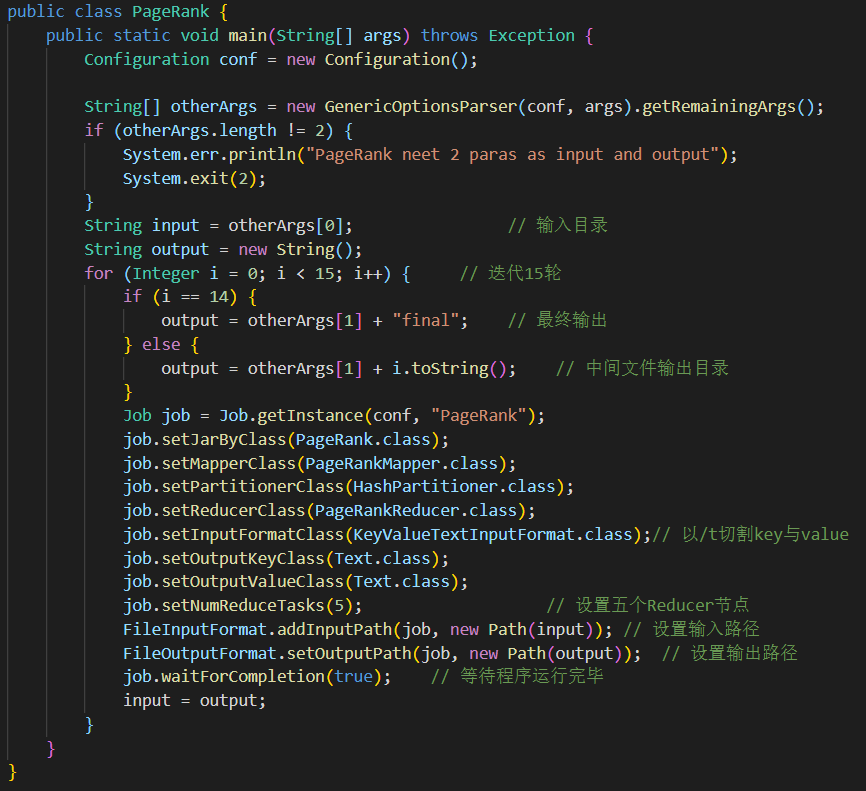
\includegraphics[width = 15cm]{PageRankMain.png}

    \caption{PageRankMain}
\end{figure}
main函数中配置指定程序运行15次,每次的结果储存在以运行次数为名的文件夹内,下一次迭代的输入为上一次的输出。

\begin{figure}[H]
    \centering

    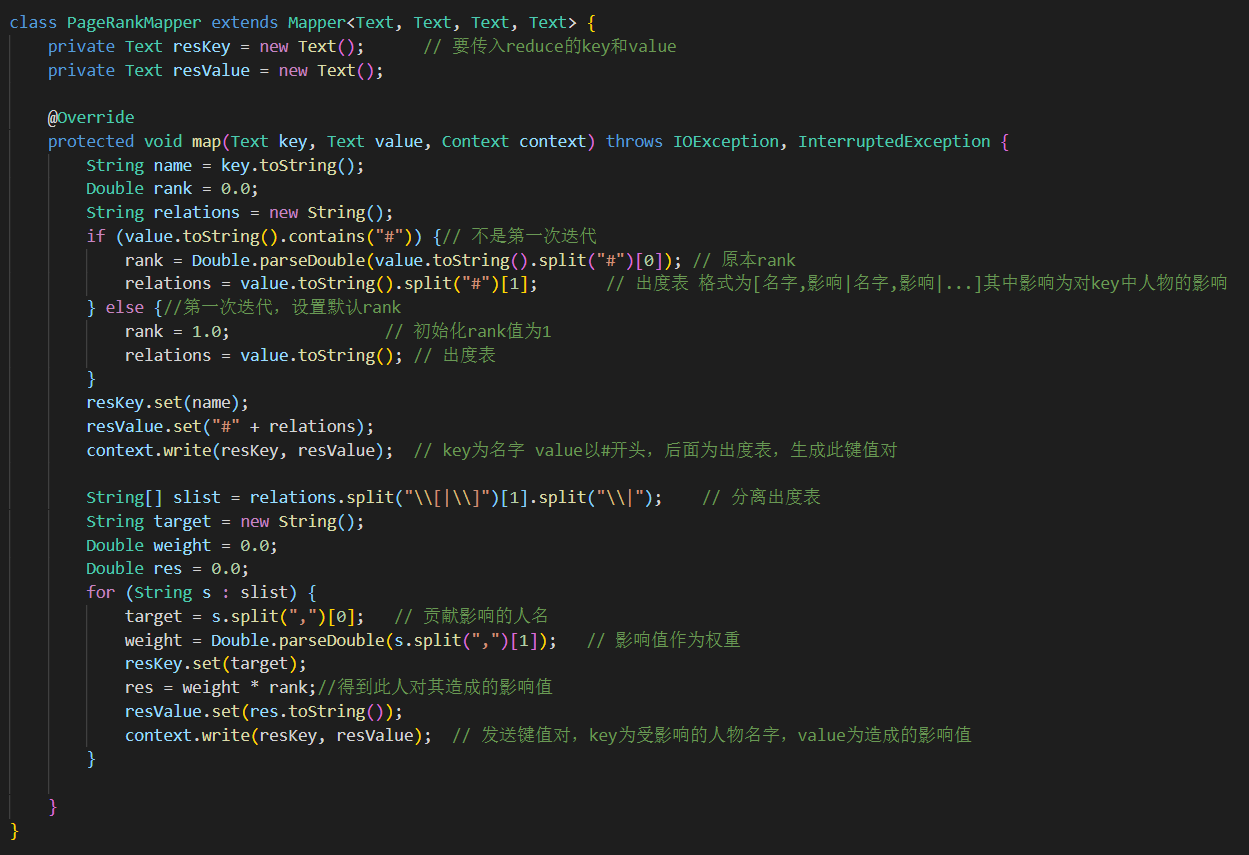
\includegraphics[width = 15cm]{PageRankMapper.png}

    \caption{PageRankReducer}
\end{figure}
Mapper阶段,首先
\begin{figure}[H]
    \centering

    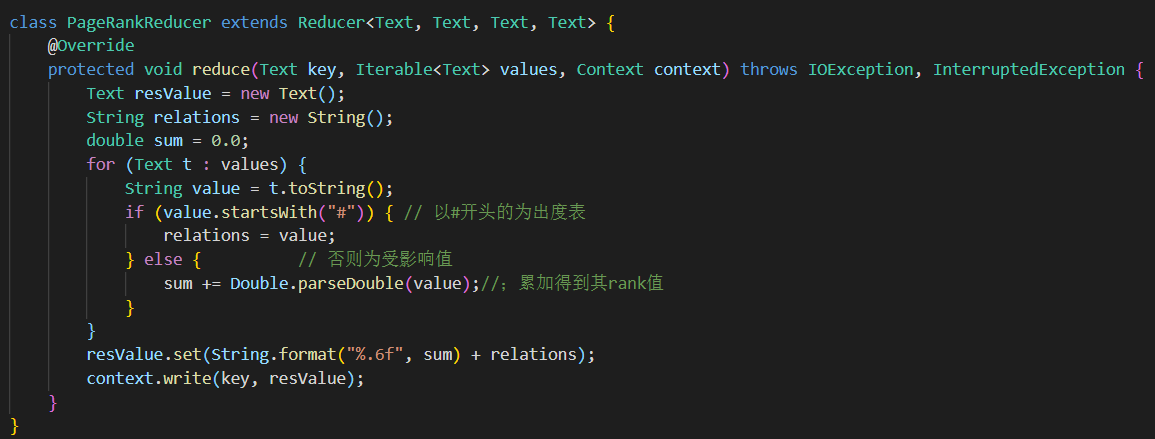
\includegraphics[width = 15cm]{PageRankReducer.png}

    \caption{PageRankReducer}
\end{figure}


\subsection{任务五}
todo

\subsection{任务六}
todo

\section{优化与改进}
\subsection{任务一}
todo

\subsection{任务二}
todo

\subsection{任务三}
todo

\subsection{任务四}
原本迭代次数为20次,在检查中间结果时发现在14次之后,结果变化不大,基本收敛,因此将迭代次数改为15次,节省开销。
\subsection{任务五}
todo

\subsection{任务六}
todo
\section{实验经验总结与改进方向}
\begin{enumerate}[1)]
    \item todo
    \item todo
\end{enumerate}
\bibliographystyle{plain}
\bibliography{ref}

\end{document}
